\subsection{Model Performance}

\begin{table}[H]
\centering
    \begin{tabular}{|l|l|l|l|l|l|l|l|l|l|l|l|l|l|l|l|l|}
        \hline
        t(s) & 0 & 1 & 2 & 3 & 4 & 5 & 6 & 7 & 8 & 9 \\ \cline{1-11} 
        predicted v(m/s) & 96.00 & 88.66 & 82.36 & 76.90 & 72.12 & 67.89 & 64.14 & 60.77 & 57.75 & 55.01
        \\ \cline{1-11}
        Actual v(m/s) & 96 & 89 & 82 & 77 & 72 & 68 & 64 & 61 & 58 & 55 \\ \cline{1-11}
        $d^2$ & 0.000 & 0.116 & 0.130 & 0.010 & 0.013 & 0.012 & 0.019 & 0.051 & 0.064 & 0.000 \\ \cline{1-11}
    \end{tabular}
    \caption{Case 1}
    \vspace{0.5cm}

    \begin{tabular}{|l|l|l|l|l|l|l|l|l|l|l|l|}
        \hline
        t(s) & 10 & 11 & 12 & 13 & 14 & 15 & 16 & 17 & 18 \\ \cline{1-10}
        predicted v(m/s) & 50.70 & 46.14 & 41.93 & 38.01 & 34.34 & 30.89 & 27.61 & 24.49 & 21.50 \\ \cline{1-10}
        Actual v(m/s) & 50 & 46 & 41 & 38 & 34 & 31 & 27 & 24 & 21 \\ \cline{1-10}
        $d^2$ & 0.484 & 0.018 & 0.858 & 0.000 & 0.118 & 0.012 & 0.377 & 0.241 & 0.247 \\ \cline{1-10}
    \end{tabular}
    \caption{Case 2}
    \vspace{0.5cm}
    
    \begin{tabular}{|l|l|l|l|l|l|l|l|l|}
        \hline
        t(s) & 19 & 20 & 21 & 22 & 23 & 24 & 25 & 26 \\ \cline{1-9}
        predicted v(m/s) & 18.61 & 15.82 & 13.10 & 10.45 & 7.84 & 5.26 & 2.71 & 0.17 \\ \cline{1-9}
        Actual v(m/s) & 18 & 16 & 13 & 10 & 8 & 5 & 3 & 0
        \\ \cline{1-9}
        $d^2$ & 0.376 & 0.032 & 0.011 & 0.199 & 0.027 & 0.069 & 0.083 & 0.030 \\ \cline{1-9}
    \end{tabular}
    \caption{Case 2 continued}
    \vspace{0.5cm}
\end{table}

\begin{figure}[H]
\centering
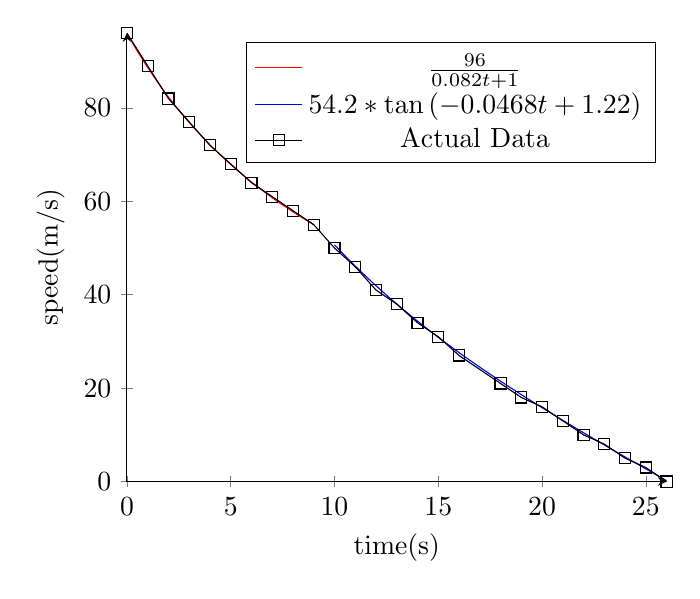
\begin{tikzpicture}
\begin{axis}[
    axis lines = left,
    xlabel = time(s),
    ylabel = speed(m/s),
]
%Below the red parabola is defined
\addplot [
    domain=0:9,
    samples=100, 
    color=red,
]
{96/(0.0828*x + 1)};
\addlegendentry{$\frac{96}{0.082t + 1}$}
%Here the blue parabloa is defined
\addplot [
    domain=10:26, 
    samples=100, 
    color=blue,
    ]
    {54.2*tan((1.22-0.0468*x)*(180/3.1415))};
\addlegendentry{$54.2*\tan{(-0.0468t+1.22)}$}
 
 \addplot[
    color=black,
    mark=square]
    coordinates {(0,96)(1,89)(2,82)(3,77)(4,72)(5,68)(6,64)(7,61)(8,58)(9,55)(10,50)(11,46)(12,41)(13,38)(14,34)(15,31)(16,27)(18,21)(19,18)(20,16)(21,13)(22,10)(23,8)(24,5)(25,3)(26,0)};
\addlegendentry{Actual Data}
\end{axis}
\end{tikzpicture}
\caption{Graph showing the predicted velocity values against the actual velocity values}
\end{figure}
